\documentclass[12pt,a4paper,oneside]{book}
% Scheletro di sorgente LaTeX per la scrittura 
% di una tesi di laurea.
% Per la grafica 
\usepackage{graphicx}
%\usepackage{forest}
%\usepackage{subcaption}
%\usepackage[]{mcode}
\usepackage{tikz}
\usetikzlibrary{matrix,chains,positioning,decorations.pathreplacing,arrows}
\usetikzlibrary{arrows,automata}
\usetikzlibrary{shapes,snakes}
\usetikzlibrary{calc,arrows}
\usetikzlibrary{scopes,matrix,positioning}
\tikzset{%	
  every neuron/.style={
    circle,
    draw,
    minimum size=0.5cm
  },
  neuron missing/.style={
    draw=none, 
    scale=3,
    text height=0.333cm,
    execute at begin node=\color{black}$\vdots$
  },
  neuron missingl/.style={
    draw=none, 
    scale=2,
    text height=0.333cm,
    execute at begin node=\color{black}$\vdots$
  },
}
\usepackage[a4paper,top=3.5cm,bottom=3cm,left=3cm,right=3cm,bindingoffset=5mm]{geometry}
%\usepackage{gensymb}
%% Per aggiungere la bibliografia nella \tableofcontents
%%\let\oldbib\bibliography
%\renewcommand{\bibliography}{\cleardoublepage1
%\addcontentsline{toc}{chapter}{\bibname}
%\oldbib}
%\usepackage[nottoc]{tocbibind}
%\onehalfspacing

%\usepackage{epigraph}

\usepackage[utf8]{inputenc}
%\usepackage[T1]{fontenc}
\usepackage{amsmath, amssymb, amsfonts}

\usepackage[pdfpagemode={UseOutlines},colorlinks=true,linktocpage=true,citecolor=blue,bookmarksnumbered=true,bookmarksopenlevel={3},pdfstartview={Fit},pdfpagelayout={SinglePage}]{hyperref}

\usepackage[english]{babel}
%\usepackage{microtype}

%\usepackage{enumitem} %personalizza liste puntate e numerate
%\setlist{leftmargin=*,nolistsep}
%\renewcommand\theenumi {\alph{enumi})}% lettere al posto di numeri
%\renewcommand\labelenumi{\theenumi}% parentesi al posto di punti


\usepackage{array}
%\usepackage{eurosym}
%\usepackage[figure]{hypcap} %link nel pdf alla figura e non alla didascalia
\usepackage{graphicx}

\usepackage{setspace}
\doublespacing
%\usepackage{emptypage}

\usepackage{fancyhdr}
%\renewcommand{\chaptermark}[1]% 
%%{\markboth{\sc{\thechapter.\ #1}}{}} 
%\renewcommand{\sectionmark}[1]%
%{\markright{\sc{\thesection.\ #1}}}

\usepackage{comment}
 
%\usepackage[
%backend=biber,
%style=alphabetic,
%sorting=ynt
%]{biblatex}

%\usepackage{biblatex}

%\addbibresource{biblio.bib}
%\bibliography{biblio.bib}


\begin{document}


%\include{tesi-cgt-frn}
\newgeometry{left=3cm,right=3cm,bottom=3cm,top=3cm}
\thispagestyle{empty}
\begin{center}

\includegraphics[height=5cm]{Figure/LOGO_UNISI.pdf}

\large{ \sc Dipartimento di ingegneria dell'informazione e scienze matematiche}
\vspace{0.5cm
\large Computer and Automation Engineering}\\
\vspace{0.5cm}
\large {\sc Robotics and Automation}
\vspace{1cm}
 
\vspace{\stretch{.8}}

%\textbf{\scshape{\LARGE{Handwritten classification of MNIST dataset\\with TensorFlow\\}}}
\textbf{\scshape{\LARGE{Closed loop approach to human-robot handshake\\}}}

\end{center}
\vspace{\stretch{1}}

\noindent\begin{minipage}[b]{0.47\textwidth}
\begin{flushleft} 
\large
\emph{Supervisor:}\\
\textit{Chiar.ssimo} \textbf{D. Prattichizzo}  
\emph{Co-supervisor:}\\
\textit{?} \textbf{M. Malvezzi}\\
\textit{?} \textbf{E. Knoop}

\end{flushleft}
\end{minipage}
\hfill
\begin{minipage}[b]{0.47\textwidth}\raggedleft
 \large
\emph{Student:}\\
\textbf{Francesco Vigni}\\


\end{minipage}

%\begin{minipage}{0.5\textwidth}
%\begin{flushright} \large
%\emph{Tesi di laurea di:} \\
%\textbf{Francesco Vigni}
%\end{flushright}
%\end{minipage}
%
%\begin{minipage}[t]{0.47\textwidth}
%{\large{\bf Relatore:\\
%Prof. NOME RELATORE}}
%\vspace{5mm}\\
%{\large{\bf Correlatore:\\
%Prof. NOME CORRELATORE\\
%Prof. NOME CORRELATORE}}\\
%%\vspace{5mm}\\
%%{\large{\bf Relatore:\\
%%Chiar.mo Prof.\\
%%NOME CORRELATORE}}
%\end{minipage}
%\hfill
%
%\begin{minipage}[t]{0.47\textwidth}\raggedleft
%{\large{\bf Candidato:\\
%NOME LAUREANDO}}
%\end{minipage}


%\noindent RELATORI:\\
%Prof. Gigi Riva\\
%Prof. alskdj
%\begin{flushright}
%TESI DI LAUREA DI:\\
%kjsad aslkjd 

%\end{flushright}
%\vspace{\stretch{1}}
%\vfill
\begin{center}
\hrule
%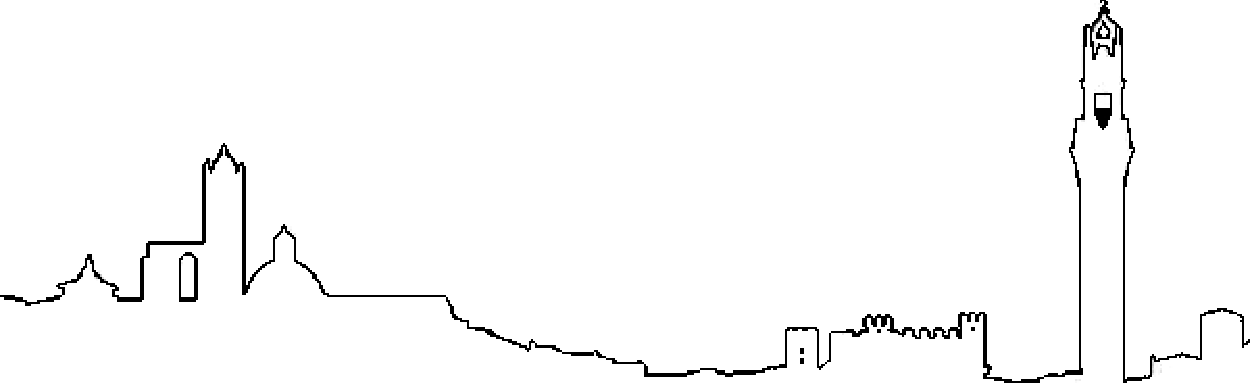
\includegraphics[width=\columnwidth]{figure/skyline1}
\vspace{0.5cm}
\large{A.A. 2017-2018}
\end{center}
\restoregeometry



\tableofcontents

%\listoffigures
%\listoftables
 

\chapter*{Introduction}
The following work wants to explore the phases of the handshake between a human and a robot, reaching a consensus in the human-machine interaction. The handshake event can be divided in two steps: the approaching and handshaking. The consensus is a parameter that allow the human to evaluate a handshake mixing aspects like: duration of the event, dynamics, force exchanged etc.. 
The handshake is the most common human-human interaction and is extensively used worldwide in events like: greetings, introduction routine between human beings and agreements. 
This work focuses only on the latter handshake step, with the purpose of evaluating different algorithms.
Many research teams focused on the the human-robot physical interaction, providing different solutions. 


\chapter{The state of the Art}
Develop a robot capable of performing a smooth human-like handshake is still a highly interested topic in the scientific literature.
A natural handshake between two humans is a very complex task to replicate, this work just focuses on the interaction force between the artificial hand and the human hand.
The consensus is a complex task to encode inside a robot, the human will always distinguish the event with respect to another human or to a robot. A human will take into consideration the skin feedback like: the temperature, the humidity and the softness. These are all characteristics that are still not embedded into the hardware available in the market. Tasks that humanoid robots can perform 

The industries are highly interested in robots since they can easily implement tasks and improve the businesses.

\cite{facialexpressions}
\cite{espen}
\cite{mirrorgame}
\cite{papageorgiou}
The robots are becoming more and more common in our daily lives, 
.
\section{}
\section{}
\section{}
\chapter{The Idea}
\chapter{Hardware setup}
\section{The Pisa/IIT qbhand}
\section{The Sensors}
\section{}
\section{Ros}


\chapter*{Conclusion}
This project applies learning \cite{art:rif.1} techniques to MNIST handwritten dataset. As we can see in the previous confusion matrix the accuracy of the final work is $97.6\%$. The overall idea is to train \emph{autoenc1},  \emph{autoenc2} and \emph{softmax1} once per time and to crop the nets in order to have coherents dimension between network interconnections. At the end of \cite{book:rif.2}this process we stack all the partial neural network together and the deep neural network come to life. \\The satisfaction behind this project can be experimented by running the file "MNIST\textunderscore drawsim.m" which is a matlab function that allows the user to draw a digit and returns the correct digit value 97,6 times over 100.

\bibliography{biblio}
\bibliographystyle{plain}

%\begin{thebibliography}{9}
%\bibitem{latexcompanion} 
%Michel Goossens, Frank Mittelbach, and Alexander Samarin. 
%\textit{The \LaTeX\ Companion}. 
%Addison-Wesley, Reading, Massachusetts, 1993.
% 
%\bibitem{einstein} 
%Albert Einstein. 
%\textit{Zur Elektrodynamik bewegter K{\"o}rper}. (German) 
%[\textit{On the electrodynamics of moving bodies}]. 
%Annalen der Physik, 322(10):891–921, 1905.
% 
%\bibitem{knuthwebsite} 
%Knuth: Computers and Typesetting,
%\\\texttt{http://www-cs-faculty.stanford.edu/\~{}uno/abcde.html}
%\end{thebibliography}
%
\end{document}
